\documentclass[a4paper, 12pt]{article}
\usepackage[T2A,T1]{fontenc}
\usepackage[utf8]{inputenc}
\usepackage[english, russian]{babel}
\usepackage{graphicx}
\usepackage[hcentering, bindingoffset = 10mm, right = 15 mm, left = 15 mm, top=20mm, bottom = 20 mm]{geometry}
\usepackage{multirow}
\usepackage{lipsum}
\usepackage{amsmath, amstext}
\usepackage{subcaption}
\usepackage{wrapfig}
\usepackage{adjustbox}
\usepackage{enumerate, indentfirst, float}
\usepackage{capt-of, svg}
\usepackage{icomma}

\newenvironment{bottompar}{\par\vspace*{\fill}}{\clearpage}

\newcommand{\LabTitle}{Магнетометр}
\begin{document}




\begin{titlepage}
\begin{center}\large
ФГАУ ВПО <<МОСКОВСКИЙ ФИЗИКО-ТЕХНИЧЕСКИЙ УНИВЕРСИТЕТ>>
\begin{figure}[H]
\centering

\includegraphics[width=15cm]{logo.jpg}
\end{figure}
{\Large
Кафедра радиотехники}

\vfill

\hrule
\vspace{0.3cm}

\huge \LabTitle

\vspace{0.3cm}
\hrule


%\noindent\rule{\textwidth}{0.4mm}
%\huge Магнитометр
%\noindent\rule{\textwidth}{0.4mm}


\end{center}

\vfill


\begin{minipage}{0.7\textwidth}
\textbf{Выполнил:}
Корепанов Г.М.

512 группа

\vspace{0.5cm}

\textbf{Преподаватель:}
Филатов Иван Васильевич
\end{minipage}


\vfill
\centering
 Долгопрудный, 2016 г.




\end{titlepage}



\section{Цель работы}
Изучение работы высокочувствительного зеркального гальванометра магнитоэлектрической системы в режимах измерения постоянного тока и электрического заряда.

В работе используются: \textit{зеркальный гальванометр с осветителем и шкалой, источник постоянного напряжения, делитель напряжения, магазин сопротивлений, эталонный конденсатор, вольтметр, переключатель, ключи, линейка.}


\subsection*{Теоретическая часть}

\begin{wrapfigure}[15]{l}{5.2cm}
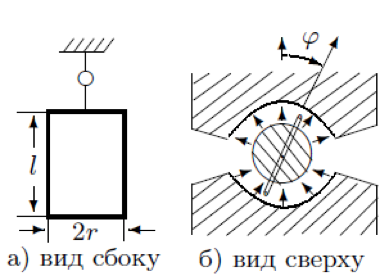
\includegraphics[width=5cm]{t}
\caption{Принцип работы}
\end{wrapfigure} 

		$$\text{Параметры установки:}$$
$$U_0,  = 1.38 \text{ В}$$
$$R_2 = 10 \text{ кОм}$$
$$R_0 = 610 \text{ Ом}$$
$$a = 136,6 \text{ см}$$
\vspace{1 cm}

\begin{equation}
J \ddot{\varphi} + \dfrac{\left(BSN\right)^2}{R_{\Sigma}} \dot{\varphi} + D\varphi = BSNI
\end{equation}
$D$ - модуль кручения нити, $\varphi$ - угол поворота рамки от положения равновесия, $B$ - индукция магнитного поля, $N$ - число витков рамки, $I$ - ток в рамке, $S$ - площадь одного витка рамки, $R_{\Sigma}$ - полное сопротивление цепи, $J$ - момент инерции подвижной системы.
Введем обозначения:

\begin{equation}
\left.
\begin{aligned}
&\dfrac{(BSN)^2}{JR_{\Sigma}} = 2\gamma \\
&\dfrac{D}{J} = \omega_0^2 \\
&\dfrac{BSN}{J} = K 
\end{aligned}
\right\}
\end{equation}

Тогда уравнение движения рамки примет вид:
\begin{equation}
\label{eq:diff}
\ddot{\varphi} +2\gamma\dot{\varphi} + \omega_0^2 \varphi = KI
\end{equation}
Величина $\gamma$ называется \textit{коэффициентом затухания} подвижной системы гальванометра,  $\omega_0$ - собственной частотой колебаний рамки.

\subsubsection*{Режим измерения постоянного тока}
При измерении в режиме постоянного тока, когда затухают колебания: $\ddot{\varphi} = \dot{\varphi} = 0$, поэтому угол поворота можно определить формулой:
$$\varphi = \dfrac{KI}{\omega_0^2} = \dfrac{I}{C_I}$$

Постоянная $C_I = D/BSN$ называется динамической постоянной гальванометра.

\subsubsection*{Свободные колебания рамки}

В отсутствии внешних источников тока ($I = 0$) будем исследовать свободное движение рамки.
Если считать, что $\varphi(0) = 0$, $\dot{\varphi} = \dot{\varphi_0}$, уравнение примет вид:
$$\ddot{\varphi} +2 \gamma \dot{\varphi} + \omega^2_0 \varphi = 0$$

общее решение такого уравнения имеет вид:
\begin{equation}
\varphi = A_1 e^{\lambda_1t} + A_2e^{\lambda_2t}
\label{eq:sol}
\end{equation}


Рассмотрим всевозможные соотношения между $\gamma$ и $\lambda$.

\begin{enumerate}

\item $\gamma < \omega_0$ (колебательный режим)

В таком случае решением уравнения \ref{eq:sol} является 
$$ \varphi = \dfrac{\dot{\varphi}}{\omega}e^{-\gamma t} \sin \omega t,$$
где $\omega^2 = \omega^2_0 - \gamma^2$
В таком режиме мы наблюдаем затухающие колебания с периодом:
$$T = \dfrac{2\pi}{\omega} = \dfrac{2 \pi}{\sqrt{\frac{D}{J} - \frac{(BSN)^4}{(2JR_\Sigma)^2}}}$$

Если $\gamma \ll \omega_0$, то $ \varphi = \dfrac{\dot{\varphi}}{\omega} \sin \omega t,$

\item $\gamma = \omega_0$ (критический режим)

Решение уравнения \ref{eq:sol} в таком случае имеет вид:
$$\varphi = \dot{\varphi	}te^{-\gamma   t}$$
Получаем, что после отклонения система экспоненциально приближается к нулю.

\item $\gamma > \omega_0$ (случай переуспокоенного гальванометра)

Решение в таком случае имеет вид:
$$ \varphi = \dfrac{\dot{\varphi}}{\sqrt{\gamma^2 - \omega_0^2}}e^{-\gamma t} \sh\sqrt{\gamma^2 - \omega_0^2}  t,$$
\end{enumerate}

\subsubsection*{Режим измерения заряда}

Момент инерции рамки искусственно увеличен, поэтому период свободных колебаний будет больше, чем время прохода короткого импульса тока. Будем считать, что рамка не изменяет своего положения при прохождении импульса.

Тогда проинтегрируем \ref{eq:diff}, домножив на $dt$ от $0$ до $\tau$ - время окончания импульса,  и получим:

$$\dot{\varphi} = K q$$
Величина $C_q = q/\varphi_{max}$ называется \textit{баллистической постоянной} гальванометра. Условия, при которых угол отклонения будет максимален при полном отсутствии затухания: $\varphi_\text{max св} = \frac{Kq}{\omega_0}$. 

В критическом режиме: 
$\varphi_\text{max кр} = \frac{Kq}{\omega_0e}$, то есть в $e$ раз меньше, чем в режиме свободных колебаний.

\section{Работа и измерения}


\subsection*{Определение динамической постоянной}

Соберем схему:

	\begin {figure}[H]
		\begin{center}
			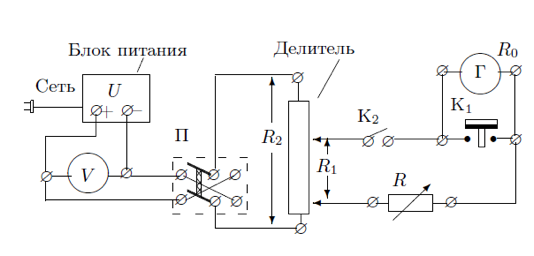
\includegraphics[width = 0.8 \textwidth]{Scheme1}
			\caption{Схема для определения динамической постоянной и критического сопротивления гальванометра}
		\end{center}
	\end {figure}

Угол отклонения рамки будем измерять с помощью осветителя, зеркальца и шкалы, находящейся на расстоянии $a$ от зеркальца. Тогда координата $x$ светового пятна будет выражаться:

$$x=a\tg(2\varphi) \approx 2a\varphi$$
Следовательно динамическая постоянная будет равна 
$$C_I = \dfrac{I}{\varphi} = \dfrac{2aI}{x}$$

Значения силы тока найдем по формуле: $$I = U_0 \dfrac{R_1}{R_2}\dfrac{1}{R+R_0}$$

% Please add the following required packages to your document preamble:
% \usepackage{graphicx}
\begin{table}[H]
\centering
\resizebox{\textwidth}{!}{%
\begin{tabular}{|l|l|l|l|l|l|l|l|l|l|l|l|l|}
\hline
$x \text{ мм}$ & 250.0 & 238.0 & 188.0 & 170.0 & 198.5 & 149.0 & 155.0 & 162.0 & 178.5 & 143.0 & 137.5 & 132.5 \\ \hline
$\sigma_x \text{ мм}$ & 1 & 1 & 1 & 1 & 1 & 1 & 1 & 1 & 1 & 1 & 1 & 1 \\ \hline
$R \text{ Ом}$ & 830.0 & 900.0 & 1300.0 & 1500.0 & 1200.0 & 1800.0 & 1700.0 & 1600.0 & 1400.0 & 1900.0 & 2000.0 & 2100.0 \\ \hline
$I \text{ нА}$ & 479.2 & 457.0 & 361.3 & 327.0 & 381.2 & 286.3 & 298.7 & 312.2 & 343.3 & 274.9 & 264.4 & 254.6 \\ \hline
$\sigma_I \text{ нА}$ & 5.4 & 5.2 & 4.5 & 4.3 & 4.7 & 4.0 & 4.1 & 4.2 & 4.4 & 3.9 & 3.8 & 3.8 \\ \hline
\end{tabular}%
}
\label{my-label}
\end{table}

% Please add the following required packages to your document preamble:
% \usepackage{graphicx}
\begin{table}[H]
\centering
\resizebox{\textwidth}{!}{%
\begin{tabular}{|l|l|l|l|l|l|l|l|l|l|l|l|l|l|l|}
\hline
127.0  & 123.0  & 119.0  & 115.5  & 112.0  & 105   & 102   & 99    & 94    & 90    & 85    & 81.5  & 78    & 73.5  & 69    \\ \hline
1      & 1      & 1      & 1      & 1      & 1     & 1     & 1     & 1     & 1     & 1     & 1     & 1     & 1     & 1     \\ \hline
2200.0 & 2300.0 & 2400.0 & 2500.0 & 2600.0 & 2800  & 2900  & 3000  & 3200  & 3400  & 3600  & 3800  & 4000  & 4300  & 4600  \\ \hline
245.6  & 237.1  & 229.2  & 221.9  & 215.0  & 202.3 & 196.6 & 191.1 & 181.1 & 172.1 & 163.9 & 156.5 & 149.7 & 140.5 & 132.4 \\ \hline
3.7    & 3.6    & 3.6    & 3.5    & 3.5    & 3.4   & 3.4   & 3.3   & 3.2   & 3.2   & 3.1   & 3.1   & 3.0   & 2.9   & 2.9   \\ \hline
\end{tabular}%
}
\label{my-label}
\end{table}

\begin{table}[H]
\resizebox{0.6\textwidth}{!}{%
\begin{tabular}{|l|l|l|l|l|l|l|l|l|l|}
\hline
64.5  & 59    & 55    & 47.5 & 42   & 38   & 29    & 25    & 21    & 14    \\ \hline
1     & 1     & 1     & 1    & 1    & 1    & 1     & 1     & 1     & 1     \\ \hline
5000  & 5500  & 6000  & 7000 & 8000 & 9000 & 12000 & 14000 & 17000 & 27000 \\ \hline
123.0 & 112.9 & 104.4 & 90.7 & 80.1 & 71.8 & 54.7  & 47.2  & 39.2  & 25.0  \\ \hline
2.8   & 2.7   & 2.7   & 2.6  & 2.5  & 2.4  & 2.3   & 2.2   & 2.1   & 2.0   \\ \hline
\end{tabular}
}
\caption{Полученные значения}
\label{my-label}
\end{table}



	\begin {figure}[H]
		\begin{center}
			% GNUPLOT: LaTeX picture with Postscript
\begingroup
  \fontfamily{sansserif}%
  \selectfont
  \makeatletter
  \providecommand\color[2][]{%
    \GenericError{(gnuplot) \space\space\space\@spaces}{%
      Package color not loaded in conjunction with
      terminal option `colourtext'%
    }{See the gnuplot documentation for explanation.%
    }{Either use 'blacktext' in gnuplot or load the package
      color.sty in LaTeX.}%
    \renewcommand\color[2][]{}%
  }%
  \providecommand\includegraphics[2][]{%
    \GenericError{(gnuplot) \space\space\space\@spaces}{%
      Package graphicx or graphics not loaded%
    }{See the gnuplot documentation for explanation.%
    }{The gnuplot epslatex terminal needs graphicx.sty or graphics.sty.}%
    \renewcommand\includegraphics[2][]{}%
  }%
  \providecommand\rotatebox[2]{#2}%
  \@ifundefined{ifGPcolor}{%
    \newif\ifGPcolor
    \GPcolorfalse
  }{}%
  \@ifundefined{ifGPblacktext}{%
    \newif\ifGPblacktext
    \GPblacktexttrue
  }{}%
  % define a \g@addto@macro without @ in the name:
  \let\gplgaddtomacro\g@addto@macro
  % define empty templates for all commands taking text:
  \gdef\gplbacktext{}%
  \gdef\gplfronttext{}%
  \makeatother
  \ifGPblacktext
    % no textcolor at all
    \def\colorrgb#1{}%
    \def\colorgray#1{}%
  \else
    % gray or color?
    \ifGPcolor
      \def\colorrgb#1{\color[rgb]{#1}}%
      \def\colorgray#1{\color[gray]{#1}}%
      \expandafter\def\csname LTw\endcsname{\color{white}}%
      \expandafter\def\csname LTb\endcsname{\color{black}}%
      \expandafter\def\csname LTa\endcsname{\color{black}}%
      \expandafter\def\csname LT0\endcsname{\color[rgb]{1,0,0}}%
      \expandafter\def\csname LT1\endcsname{\color[rgb]{0,1,0}}%
      \expandafter\def\csname LT2\endcsname{\color[rgb]{0,0,1}}%
      \expandafter\def\csname LT3\endcsname{\color[rgb]{1,0,1}}%
      \expandafter\def\csname LT4\endcsname{\color[rgb]{0,1,1}}%
      \expandafter\def\csname LT5\endcsname{\color[rgb]{1,1,0}}%
      \expandafter\def\csname LT6\endcsname{\color[rgb]{0,0,0}}%
      \expandafter\def\csname LT7\endcsname{\color[rgb]{1,0.3,0}}%
      \expandafter\def\csname LT8\endcsname{\color[rgb]{0.5,0.5,0.5}}%
    \else
      % gray
      \def\colorrgb#1{\color{black}}%
      \def\colorgray#1{\color[gray]{#1}}%
      \expandafter\def\csname LTw\endcsname{\color{white}}%
      \expandafter\def\csname LTb\endcsname{\color{black}}%
      \expandafter\def\csname LTa\endcsname{\color{black}}%
      \expandafter\def\csname LT0\endcsname{\color{black}}%
      \expandafter\def\csname LT1\endcsname{\color{black}}%
      \expandafter\def\csname LT2\endcsname{\color{black}}%
      \expandafter\def\csname LT3\endcsname{\color{black}}%
      \expandafter\def\csname LT4\endcsname{\color{black}}%
      \expandafter\def\csname LT5\endcsname{\color{black}}%
      \expandafter\def\csname LT6\endcsname{\color{black}}%
      \expandafter\def\csname LT7\endcsname{\color{black}}%
      \expandafter\def\csname LT8\endcsname{\color{black}}%
    \fi
  \fi
    \setlength{\unitlength}{0.0500bp}%
    \ifx\gptboxheight\undefined%
      \newlength{\gptboxheight}%
      \newlength{\gptboxwidth}%
      \newsavebox{\gptboxtext}%
    \fi%
    \setlength{\fboxrule}{0.5pt}%
    \setlength{\fboxsep}{1pt}%
\begin{picture}(9354.00,6802.00)%
    \gplgaddtomacro\gplbacktext{%
      \csname LTb\endcsname%
      \put(660,1408){\makebox(0,0)[r]{\strut{}$0$}}%
      \csname LTb\endcsname%
      \put(660,2381){\makebox(0,0)[r]{\strut{}$100$}}%
      \csname LTb\endcsname%
      \put(660,3354){\makebox(0,0)[r]{\strut{}$200$}}%
      \csname LTb\endcsname%
      \put(660,4327){\makebox(0,0)[r]{\strut{}$300$}}%
      \csname LTb\endcsname%
      \put(660,5300){\makebox(0,0)[r]{\strut{}$400$}}%
      \csname LTb\endcsname%
      \put(660,6273){\makebox(0,0)[r]{\strut{}$500$}}%
      \csname LTb\endcsname%
      \put(924,968){\makebox(0,0){\strut{}$0$}}%
      \csname LTb\endcsname%
      \put(2604,968){\makebox(0,0){\strut{}$50$}}%
      \csname LTb\endcsname%
      \put(4285,968){\makebox(0,0){\strut{}$100$}}%
      \csname LTb\endcsname%
      \put(5965,968){\makebox(0,0){\strut{}$150$}}%
      \csname LTb\endcsname%
      \put(7646,968){\makebox(0,0){\strut{}$200$}}%
      \csname LTb\endcsname%
      \put(9326,968){\makebox(0,0){\strut{}$250$}}%
      \put(1764,5787){\makebox(0,0)[l]{\strut{}$K = \left(1.927\pm0.02\right)$ нА/мм}}%
    }%
    \gplgaddtomacro\gplfronttext{%
      \csname LTb\endcsname%
      \put(-9,3840){\rotatebox{-270}{\makebox(0,0){\strut{}$I$, нА}}}%
      \put(5125,308){\makebox(0,0){\strut{}$x$, мм}}%
    }%
    \gplbacktext
    \put(0,0){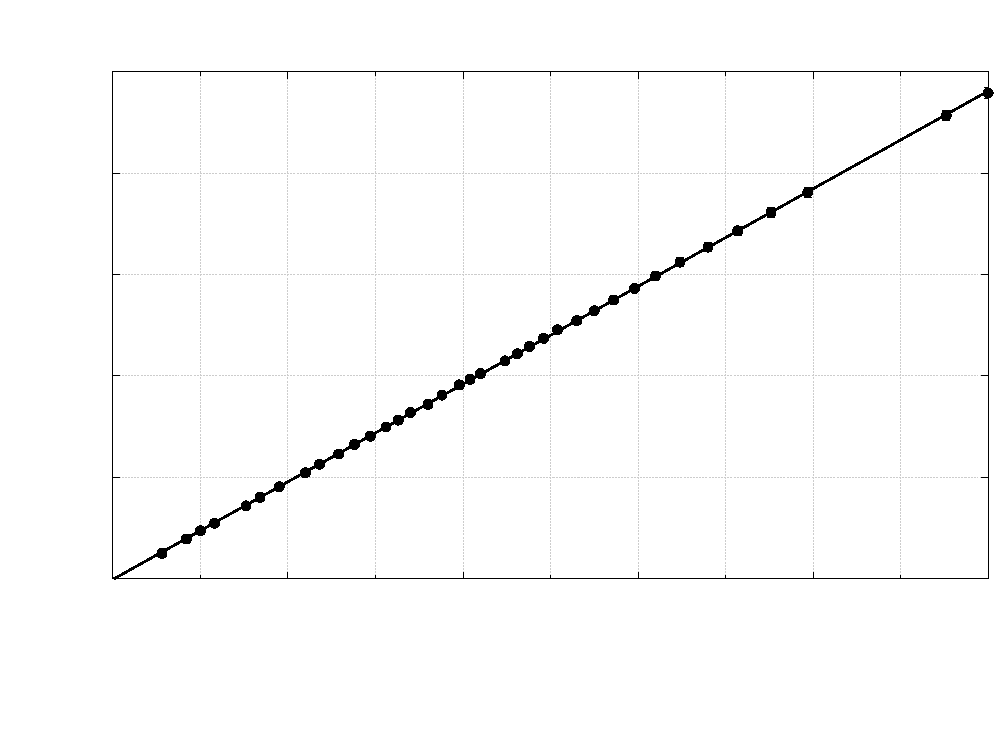
\includegraphics{plot1}}%
    \gplfronttext
  \end{picture}%
\endgroup

			\caption{График зависимости $I = f(x)$}
		\end{center}
	\end {figure}

Получаем, что $\dfrac{C_I}{2a} = 1,927\pm 0,02 \; \dfrac{\text{нА}}{\text{ мм}}$

Тогда $C_I = 5.27 \pm 0.05 \; \dfrac{\text{нА}}{\text{ мм$/$м}}$
	
\subsection*{Определение критического сопротивления}
$$x_n = 249 \text{ мм}$$
$$x_{n+1} = 220 \text{ мм}$$
$$\Theta_0 \simeq \ln \dfrac{x_n}{x_{n+1}} = 0.12$$	
Оценим примерное значение периода свободных колебаний:
\begin{table}[H]
\centering
\begin{tabular}{|l|l|l|}
\hline
$t$, с   & 66.9 & 66.9 \\ \hline
$N$, раз & 27.0 & 27.0 \\ \hline
$T$, с   & 2.5  & 2.5  \\ \hline
\end{tabular}
\caption{Определение периода}
\label{my-label}
\end{table}
$$T_0 = 2.48 \pm 0.04 \text{ с}$$
Оценим значение критического сопротивления, при котором зайчик не переходит за нулевое значение:
$$R_{\text{кр}} \approx 4330 \text{ Ом}$$

% Please add the following required packages to your document preamble:
% \usepackage{graphicx}
\begin{table}[H]
\centering
\resizebox{\textwidth}{!}{%
\begin{tabular}{|l|l|l|l|l|l|l|l|l|}
\hline
\textbf{$R/R_\text{ кр}$} & \textbf{$R, \text{ кОм}$} & \textbf{$x_n$, мм} & \textbf{$x_{n+1}$, мм} & \textbf{$\Theta$} & \textbf{$\sigma_ \Theta$} & \textbf{$1/\Theta^2$} & \textbf{$\sigma _{\theta^ 2}$} & \textbf{$(R+R_0)^2 \text{ кОм}^2$} \\ \hline
3.00                      & 13.0                      & 222.0              & 22.0                   & 2.31              & 0.25                 & 0.19                  & 0.04                                   & 185.0                              \\ \hline
3.50                      & 15.2                      & 192.0              & 26.0                   & 2.00              & 0.16                 & 0.25                  & 0.04                                   & 248.5                              \\ \hline
4.00                      & 17.3                      & 224.0              & 39.0                   & 1.75              & 0.09                 & 0.33                  & 0.03                                   & 321.5                              \\ \hline
4.50                      & 19.5                      & 200.0              & 41.0                   & 1.58              & 0.07                 & 0.40                  & 0.04                                   & 403.8                              \\ \hline
5.01                      & 21.7                      & 180.0              & 43.0                   & 1.43              & 0.06                 & 0.49                  & 0.04                                   & 497.7                              \\ \hline
5.50                      & 23.8                      & 245.0              & 64.0                   & 1.34              & 0.04                 & 0.55                  & 0.03                                   & 596.6                              \\ \hline
6.00                      & 26.0                      & 225.0              & 67.0                   & 1.21              & 0.03                 & 0.68                  & 0.04                                   & 707.0                              \\ \hline
7.00                      & 30.3                      & 193.0              & 67.0                   & 1.06              & 0.03                 & 0.89                  & 0.05                                   & 956.0                              \\ \hline
8.00                      & 34.6                      & 241.0              & 94.0                   & 0.94              & 0.02                 & 1.13                  & 0.05                                   & 1242.6                             \\ \hline
9.00                      & 39.0                      & 215.0              & 92.0                   & 0.85              & 0.02                 & 1.39                  & 0.06                                   & 1566.6                             \\ \hline
10.00                     & 43.3                      & 194.0              & 89.0                   & 0.78              & 0.02                 & 1.65                  & 0.08                                   & 1928.1                             \\ \hline
\end{tabular}%
}
\caption{Исследование зависимости $\Theta$ от $R$}
\label{my-label}
\end{table}

\begin{equation}
\Theta = \gamma T = 2 \pi \dfrac{\gamma}{\omega} = \dfrac{2 \pi \gamma}{\sqrt{\omega_0^2 - \gamma^2}} = \dfrac{2 \pi R_3}{\sqrt{R_\Sigma^2 - R_3^2}},
\label{eq:critical}
\end{equation}
где введено обозначение:
$$R_3 = \frac{(BSN)^2}{2\sqrt{JD}} = R_0 + R_\text{кр}$$
Тогда при $R = R_\text{кр}$  выполняется: $\Theta \rightarrow \infty$

Получим из \ref{eq:critical} уравнение прямой в координатах $X = (R_0 + R)^2$ и $Y = 1/\Theta^2$:

$$\dfrac{1}{\Theta^2} = \dfrac{(R_0 + R)^2}{4 \pi^2 R_3^2} - \dfrac{1}{4 \pi^2}$$

Тогда $R_\text{кр} = \dfrac{1}{2 \pi} \sqrt{\dfrac{\Delta X}{\Delta Y}} - R_0$

\begin {figure}[H]
	\begin{center}
% GNUPLOT: LaTeX picture with Postscript
\begingroup
  \fontfamily{sansserif}%
  \selectfont
  \makeatletter
  \providecommand\color[2][]{%
    \GenericError{(gnuplot) \space\space\space\@spaces}{%
      Package color not loaded in conjunction with
      terminal option `colourtext'%
    }{See the gnuplot documentation for explanation.%
    }{Either use 'blacktext' in gnuplot or load the package
      color.sty in LaTeX.}%
    \renewcommand\color[2][]{}%
  }%
  \providecommand\includegraphics[2][]{%
    \GenericError{(gnuplot) \space\space\space\@spaces}{%
      Package graphicx or graphics not loaded%
    }{See the gnuplot documentation for explanation.%
    }{The gnuplot epslatex terminal needs graphicx.sty or graphics.sty.}%
    \renewcommand\includegraphics[2][]{}%
  }%
  \providecommand\rotatebox[2]{#2}%
  \@ifundefined{ifGPcolor}{%
    \newif\ifGPcolor
    \GPcolorfalse
  }{}%
  \@ifundefined{ifGPblacktext}{%
    \newif\ifGPblacktext
    \GPblacktexttrue
  }{}%
  % define a \g@addto@macro without @ in the name:
  \let\gplgaddtomacro\g@addto@macro
  % define empty templates for all commands taking text:
  \gdef\gplbacktext{}%
  \gdef\gplfronttext{}%
  \makeatother
  \ifGPblacktext
    % no textcolor at all
    \def\colorrgb#1{}%
    \def\colorgray#1{}%
  \else
    % gray or color?
    \ifGPcolor
      \def\colorrgb#1{\color[rgb]{#1}}%
      \def\colorgray#1{\color[gray]{#1}}%
      \expandafter\def\csname LTw\endcsname{\color{white}}%
      \expandafter\def\csname LTb\endcsname{\color{black}}%
      \expandafter\def\csname LTa\endcsname{\color{black}}%
      \expandafter\def\csname LT0\endcsname{\color[rgb]{1,0,0}}%
      \expandafter\def\csname LT1\endcsname{\color[rgb]{0,1,0}}%
      \expandafter\def\csname LT2\endcsname{\color[rgb]{0,0,1}}%
      \expandafter\def\csname LT3\endcsname{\color[rgb]{1,0,1}}%
      \expandafter\def\csname LT4\endcsname{\color[rgb]{0,1,1}}%
      \expandafter\def\csname LT5\endcsname{\color[rgb]{1,1,0}}%
      \expandafter\def\csname LT6\endcsname{\color[rgb]{0,0,0}}%
      \expandafter\def\csname LT7\endcsname{\color[rgb]{1,0.3,0}}%
      \expandafter\def\csname LT8\endcsname{\color[rgb]{0.5,0.5,0.5}}%
    \else
      % gray
      \def\colorrgb#1{\color{black}}%
      \def\colorgray#1{\color[gray]{#1}}%
      \expandafter\def\csname LTw\endcsname{\color{white}}%
      \expandafter\def\csname LTb\endcsname{\color{black}}%
      \expandafter\def\csname LTa\endcsname{\color{black}}%
      \expandafter\def\csname LT0\endcsname{\color{black}}%
      \expandafter\def\csname LT1\endcsname{\color{black}}%
      \expandafter\def\csname LT2\endcsname{\color{black}}%
      \expandafter\def\csname LT3\endcsname{\color{black}}%
      \expandafter\def\csname LT4\endcsname{\color{black}}%
      \expandafter\def\csname LT5\endcsname{\color{black}}%
      \expandafter\def\csname LT6\endcsname{\color{black}}%
      \expandafter\def\csname LT7\endcsname{\color{black}}%
      \expandafter\def\csname LT8\endcsname{\color{black}}%
    \fi
  \fi
    \setlength{\unitlength}{0.0500bp}%
    \ifx\gptboxheight\undefined%
      \newlength{\gptboxheight}%
      \newlength{\gptboxwidth}%
      \newsavebox{\gptboxtext}%
    \fi%
    \setlength{\fboxrule}{0.5pt}%
    \setlength{\fboxsep}{1pt}%
\begin{picture}(9354.00,6802.00)%
    \gplgaddtomacro\gplbacktext{%
      \csname LTb\endcsname%
      \put(660,1408){\makebox(0,0)[r]{\strut{}$0$}}%
      \csname LTb\endcsname%
      \put(660,2103){\makebox(0,0)[r]{\strut{}$1$}}%
      \csname LTb\endcsname%
      \put(660,2798){\makebox(0,0)[r]{\strut{}$2$}}%
      \csname LTb\endcsname%
      \put(660,3493){\makebox(0,0)[r]{\strut{}$3$}}%
      \csname LTb\endcsname%
      \put(660,4188){\makebox(0,0)[r]{\strut{}$4$}}%
      \csname LTb\endcsname%
      \put(660,4883){\makebox(0,0)[r]{\strut{}$5$}}%
      \csname LTb\endcsname%
      \put(660,5578){\makebox(0,0)[r]{\strut{}$6$}}%
      \csname LTb\endcsname%
      \put(660,6273){\makebox(0,0)[r]{\strut{}$7$}}%
      \csname LTb\endcsname%
      \put(924,968){\makebox(0,0){\strut{}$0$}}%
      \csname LTb\endcsname%
      \put(2324,968){\makebox(0,0){\strut{}$1$}}%
      \csname LTb\endcsname%
      \put(3725,968){\makebox(0,0){\strut{}$2$}}%
      \csname LTb\endcsname%
      \put(5125,968){\makebox(0,0){\strut{}$3$}}%
      \csname LTb\endcsname%
      \put(6525,968){\makebox(0,0){\strut{}$4$}}%
      \csname LTb\endcsname%
      \put(7926,968){\makebox(0,0){\strut{}$5$}}%
      \csname LTb\endcsname%
      \put(9326,968){\makebox(0,0){\strut{}$6$}}%
    }%
    \gplgaddtomacro\gplfronttext{%
      \csname LTb\endcsname%
      \put(176,3840){\rotatebox{-270}{\makebox(0,0){\strut{}$\tg\varphi$}}}%
      \put(5125,308){\makebox(0,0){\strut{}$1/\omega R_{\sum} C$}}%
    }%
    \gplbacktext
    \put(0,0){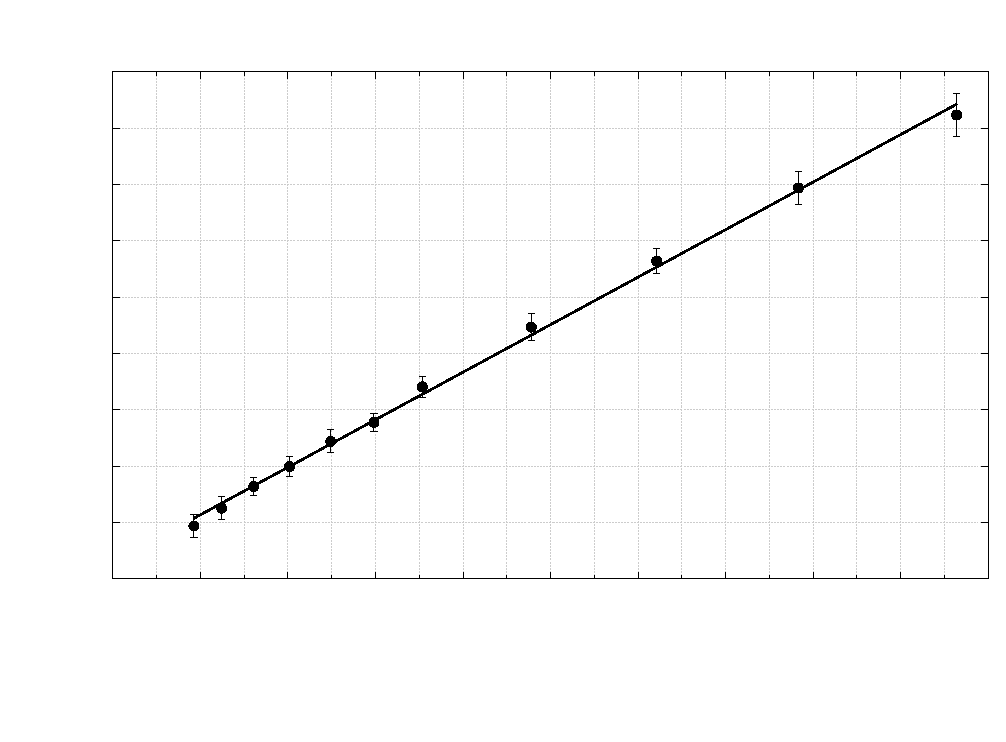
\includegraphics{plot2}}%
    \gplfronttext
  \end{picture}%
\endgroup

		\caption{График зависимости $1/\Theta^2 = f((R_0 + R)^2)$}
	\end{center}
\end {figure}


Из графика $\dfrac{\Delta X}{\Delta Y} = 11.8 \pm 0.6 \text{ (10 кОм)}^2$, поэтому 
$$R_\text{кр} = 4.85 \pm 0.12 \text{  кОм}$$

\subsection*{Баллистический режим}

$$C = 2 \text{ мкФ}$$
$$R_1/R_2 = 1/15$$
$$l_{max} = 19,4 \text{ см}$$
$$l_{\text{своб}} = l_{max} \cdot e^{\theta_0/4}=20,0 \text{ см}$$

Соберем схему:

\begin {figure}[H]
	\begin{center}
		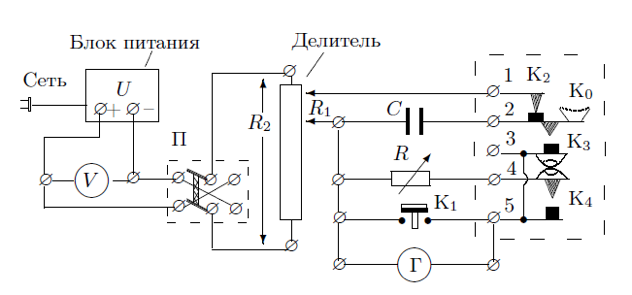
\includegraphics[width = 0.8 \textwidth]{Scheme2}
		\caption{Схема для определения баллистической постоянной и критического сопротивления гальванометра, работающего в баллистическом режиме}
	\end{center}
\end {figure}

%\begin{table}[H]
%\centering
%\begin{tabular}{|c|c|c|c|}
%\hline
%$R, \text{ Ом}$ & $l_{max}$ & $\sigma_{l_{max}}$ & $(R+R_0)^{-1}, \; 10^6 \; \text{Ом}^{-1}$ \\ \hline
%30000.0         & 13.6      & 0.4                & 3.3            \\ \hline
%25000.0         & 13.2      & 0.4                & 3.9            \\ \hline
%20000.0         & 12.8      & 0.4                & 4.9            \\ \hline
%15000.0         & 11.6      & 0.4                & 6.4            \\ \hline
%10000.0         & 9.5       & 0.4                & 9.4            \\ \hline
%9000.0          & 9.3       & 0.4                & 10.4           \\ \hline
%8000.0          & 8.8       & 0.4                & 11.6           \\ \hline
%7000.0          & 8.2       & 0.4                & 13.1           \\ \hline
%6000.0          & 7.7       & 0.4                & 15.1           \\ \hline
%5000.0          & 6.9       & 0.4                & 17.8           \\ \hline
%\end{tabular}
%\caption{Исследуем зависимость между $l_{max}$ и $R$}
%\end{table}

\begin {figure}[H]
	\begin{center}
		% GNUPLOT: LaTeX picture with Postscript
\begingroup
  \fontfamily{sansserif}%
  \selectfont
  \makeatletter
  \providecommand\color[2][]{%
    \GenericError{(gnuplot) \space\space\space\@spaces}{%
      Package color not loaded in conjunction with
      terminal option `colourtext'%
    }{See the gnuplot documentation for explanation.%
    }{Either use 'blacktext' in gnuplot or load the package
      color.sty in LaTeX.}%
    \renewcommand\color[2][]{}%
  }%
  \providecommand\includegraphics[2][]{%
    \GenericError{(gnuplot) \space\space\space\@spaces}{%
      Package graphicx or graphics not loaded%
    }{See the gnuplot documentation for explanation.%
    }{The gnuplot epslatex terminal needs graphicx.sty or graphics.sty.}%
    \renewcommand\includegraphics[2][]{}%
  }%
  \providecommand\rotatebox[2]{#2}%
  \@ifundefined{ifGPcolor}{%
    \newif\ifGPcolor
    \GPcolorfalse
  }{}%
  \@ifundefined{ifGPblacktext}{%
    \newif\ifGPblacktext
    \GPblacktexttrue
  }{}%
  % define a \g@addto@macro without @ in the name:
  \let\gplgaddtomacro\g@addto@macro
  % define empty templates for all commands taking text:
  \gdef\gplbacktext{}%
  \gdef\gplfronttext{}%
  \makeatother
  \ifGPblacktext
    % no textcolor at all
    \def\colorrgb#1{}%
    \def\colorgray#1{}%
  \else
    % gray or color?
    \ifGPcolor
      \def\colorrgb#1{\color[rgb]{#1}}%
      \def\colorgray#1{\color[gray]{#1}}%
      \expandafter\def\csname LTw\endcsname{\color{white}}%
      \expandafter\def\csname LTb\endcsname{\color{black}}%
      \expandafter\def\csname LTa\endcsname{\color{black}}%
      \expandafter\def\csname LT0\endcsname{\color[rgb]{1,0,0}}%
      \expandafter\def\csname LT1\endcsname{\color[rgb]{0,1,0}}%
      \expandafter\def\csname LT2\endcsname{\color[rgb]{0,0,1}}%
      \expandafter\def\csname LT3\endcsname{\color[rgb]{1,0,1}}%
      \expandafter\def\csname LT4\endcsname{\color[rgb]{0,1,1}}%
      \expandafter\def\csname LT5\endcsname{\color[rgb]{1,1,0}}%
      \expandafter\def\csname LT6\endcsname{\color[rgb]{0,0,0}}%
      \expandafter\def\csname LT7\endcsname{\color[rgb]{1,0.3,0}}%
      \expandafter\def\csname LT8\endcsname{\color[rgb]{0.5,0.5,0.5}}%
    \else
      % gray
      \def\colorrgb#1{\color{black}}%
      \def\colorgray#1{\color[gray]{#1}}%
      \expandafter\def\csname LTw\endcsname{\color{white}}%
      \expandafter\def\csname LTb\endcsname{\color{black}}%
      \expandafter\def\csname LTa\endcsname{\color{black}}%
      \expandafter\def\csname LT0\endcsname{\color{black}}%
      \expandafter\def\csname LT1\endcsname{\color{black}}%
      \expandafter\def\csname LT2\endcsname{\color{black}}%
      \expandafter\def\csname LT3\endcsname{\color{black}}%
      \expandafter\def\csname LT4\endcsname{\color{black}}%
      \expandafter\def\csname LT5\endcsname{\color{black}}%
      \expandafter\def\csname LT6\endcsname{\color{black}}%
      \expandafter\def\csname LT7\endcsname{\color{black}}%
      \expandafter\def\csname LT8\endcsname{\color{black}}%
    \fi
  \fi
    \setlength{\unitlength}{0.0500bp}%
    \ifx\gptboxheight\undefined%
      \newlength{\gptboxheight}%
      \newlength{\gptboxwidth}%
      \newsavebox{\gptboxtext}%
    \fi%
    \setlength{\fboxrule}{0.5pt}%
    \setlength{\fboxsep}{1pt}%
\begin{picture}(9354.00,6802.00)%
    \gplgaddtomacro\gplbacktext{%
      \csname LTb\endcsname%
      \put(660,1408){\makebox(0,0)[r]{\strut{}$40$}}%
      \csname LTb\endcsname%
      \put(660,2016){\makebox(0,0)[r]{\strut{}$60$}}%
      \csname LTb\endcsname%
      \put(660,2624){\makebox(0,0)[r]{\strut{}$80$}}%
      \csname LTb\endcsname%
      \put(660,3232){\makebox(0,0)[r]{\strut{}$100$}}%
      \csname LTb\endcsname%
      \put(660,3841){\makebox(0,0)[r]{\strut{}$120$}}%
      \csname LTb\endcsname%
      \put(660,4449){\makebox(0,0)[r]{\strut{}$140$}}%
      \csname LTb\endcsname%
      \put(660,5057){\makebox(0,0)[r]{\strut{}$160$}}%
      \csname LTb\endcsname%
      \put(660,5665){\makebox(0,0)[r]{\strut{}$180$}}%
      \csname LTb\endcsname%
      \put(660,6273){\makebox(0,0)[r]{\strut{}$200$}}%
      \csname LTb\endcsname%
      \put(924,968){\makebox(0,0){\strut{}$0$}}%
      \csname LTb\endcsname%
      \put(2324,968){\makebox(0,0){\strut{}$50$}}%
      \csname LTb\endcsname%
      \put(3725,968){\makebox(0,0){\strut{}$100$}}%
      \csname LTb\endcsname%
      \put(5125,968){\makebox(0,0){\strut{}$150$}}%
      \csname LTb\endcsname%
      \put(6525,968){\makebox(0,0){\strut{}$200$}}%
      \csname LTb\endcsname%
      \put(7926,968){\makebox(0,0){\strut{}$250$}}%
      \csname LTb\endcsname%
      \put(9326,968){\makebox(0,0){\strut{}$300$}}%
    }%
    \gplgaddtomacro\gplfronttext{%
      \csname LTb\endcsname%
      \put(-9,3840){\rotatebox{-270}{\makebox(0,0){\strut{}$l_{max}$, мм}}}%
      \put(5125,308){\makebox(0,0){\strut{}$1/(R+R_0)$, $10^{-6} \text{ Ом}^{-1}$}}%
    }%
    \gplbacktext
    \put(0,0){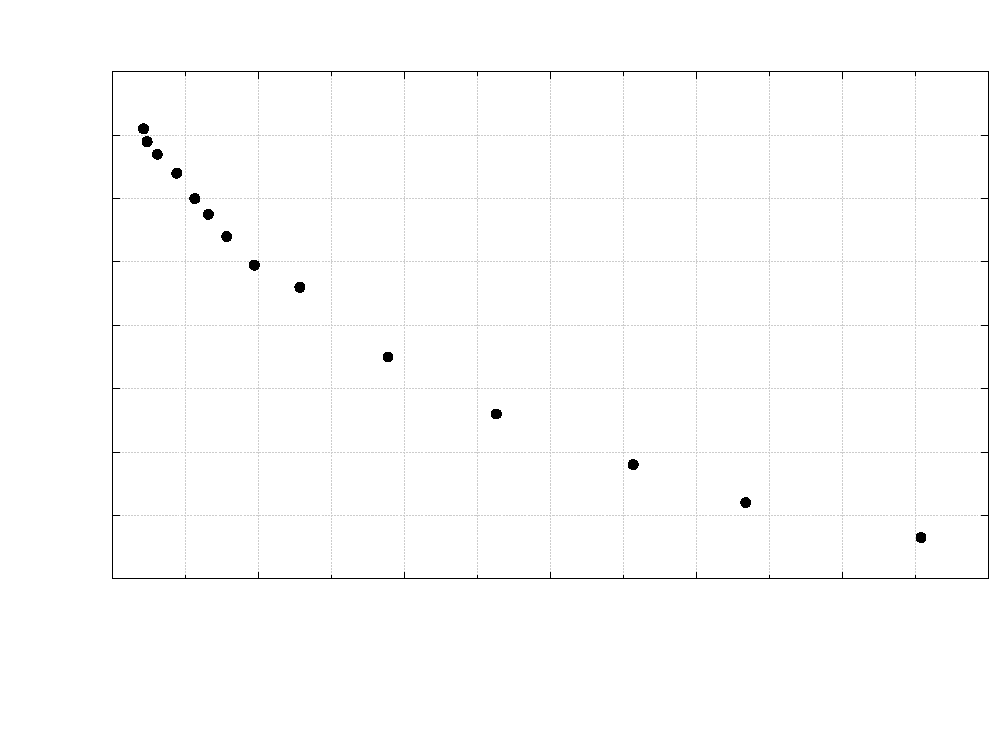
\includegraphics{plot3}}%
    \gplfronttext
  \end{picture}%
\endgroup

		\caption{Зависимость $l_{max} = f[(R_0+R)^{-1}]$}
	\end{center}
\end {figure}

Определим значение $R_\text{кр}$ по графику: значение максимального отклонения в критическом режиме в $e$ раз меньше, чем в режиме свободных колебаний. Зная зависимость $l_{max} = f[(R_0+R)^{-1}]$ найдем значение сопротивления, соответствующее 
$$R_\text{кр} = R(l_{\text{своб}}/e) = $$

Определим баллистическую постоянную гальванометра $C_{Q_\text{кр}} \left[\dfrac{\text{Кл}}{\text{мм/м}} \right]$:

$$C_{Q_\text{кр}} = \dfrac{q}{\varphi_{max \text{ кр}}} = 2a \dfrac{R_1}{R_2} \dfrac{U_0C}{l_{max \text{ кр}}} = $$

Время релаксации $t = R_0C = 610 \cdot 2 \cdot 10^{-6} = 1.22 \cdot 10^{-3} \text{ с} \ll T_0 = 2.48 \text{ с}$

\section{Вывод}

В данной лабораторной работе мы измерили значение динамической постоянной гальванометра, критического сопротивления тремя способами и баллистической постоянной. В измерениях динамической постоянной значения $R_\text{кр}$ совпадают с учетом погрешности. Наибольшая погрешность в третьем эксперименте, так как большой вклад в погрешность дает скорость реакции человека (отклонения зайчика происходят быстро, необходимо успевать замыкать ключ и считывать значения).

\end{document}